\chapter{Hierarchical Approximate Convex Decomposition}\label{sec:hacd}
\section{Implementation}
Bullet 2.83 contain a
composite (or compound) shape, a shape container which contain sub-shapes and act
as a joint rigid body. Bullet updates the inertia of the object internally as
more sub-shapes are added, as well as the bounding box needed for the SAP.

An implementation of HACD is included with Bullet's source code and the code is
developed by Mamou and based on the work of~\cite{mamou}. Some input parameters are available, these have been
left as the recommended parameters. The parameters control for instance, concavity
penalty weights, (i.e if you can disregard a small concavity)
and the maximum amount of points per convex hull.
The method while effective in terms of convex decomposition can not be described as
particularly effective in terms of performance. A Utah Teapot of around 4300 vertices,
takes approximately 25 seconds to decompose. The method is in addition rotationally
 variant, so results may vary depending on the rotation of the object which is to be decomposed.

 \begin{figure}[H]
   \centering
   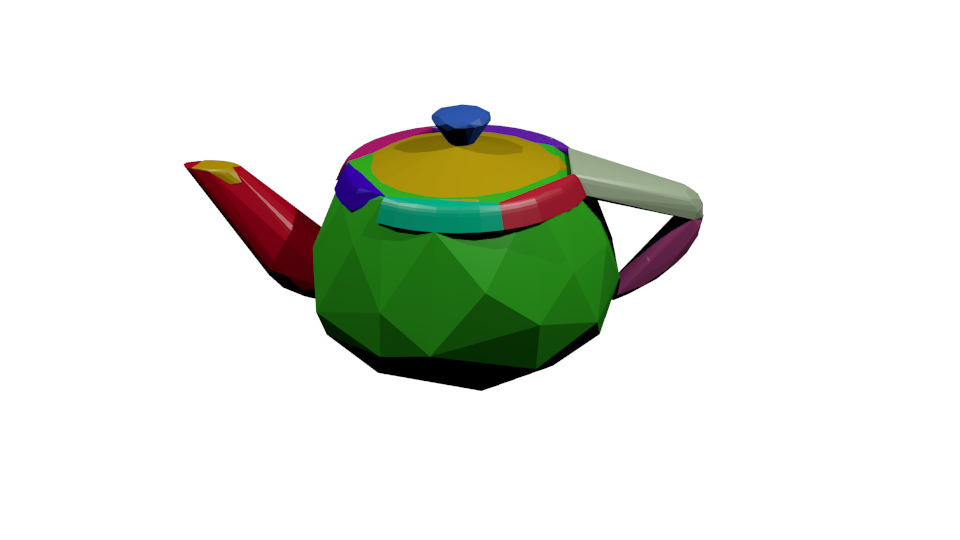
\includegraphics[width = 0.8\textwidth]{hacdTeapot.png}
   \caption{The decomposition from HACD method, model left in initial orientation}
   \label{fig:HACD}
 \end{figure}

The models are added in a three dimensional grid above the bin and the simulation
is started. In figure~\ref{fig:hacdStart} is a figure of the start position.

\begin{figure}[H]
  \centering
  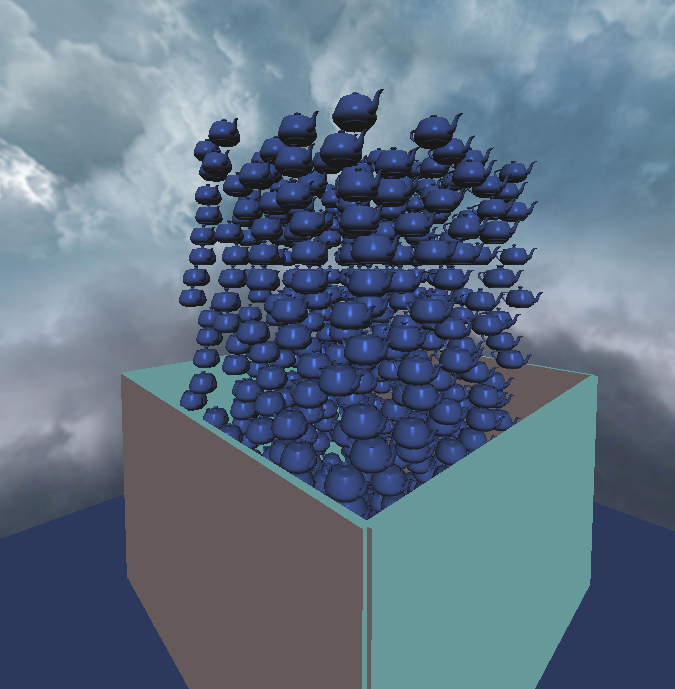
\includegraphics[width = 0.8\textwidth]{HACDstart05-11.png}
  \caption{The inital state of the simulation}
  \label{fig:hacdStart}
\end{figure}

During a simulation much more time is spent in the last
part of the simulation when most of the models are quite stationary and only small
changes are made. The increased frametime in the later parts of the simulation is
due to the many contacts between the objects. A lot of small rolling motions, likely due to the round
shape of the Utah Teapot can be observed. Without the small rolling effect Bullet's
sleeping would take effect earlier and increase performance. One can expect that
more rectangular objects to have better performance.

\section{Performance}
For testing, a Utah teapot consisting of 12 submodels were used. Each submodel have
between 50 and 100 vertices. A timestep of 0.01 seconds were used. All timings
presented are without rendering. All tests measure simulation
time and averages the result across 2000 iterations. For the first test, Bullets' sleeping was
disabled and the second the sleeping was left enabled. The results are presented
in table~\ref{tab:hacdtest}.

\begin{table}[htbp]
\caption{Testing of Bullet with HACD}
\begin{center}
\begin{tabular}{|l|r|r|}
\hline
\textbf{Sleeping Enabled} & \multicolumn{1}{l|}{\textbf{Number of objects}} & \multicolumn{1}{l|}{\textbf{Time/frame [ms]}} \\ \hline
No & 512 & 51,9156 \\ \hline
Yes  & 512 & 30,5515 \\ \hline
No & 256 & 22,3175 \\ \hline
Yes  & 256 & 13,298 \\ \hline
\end{tabular}
\end{center}
\label{tab:hacdtest}
\end{table}

\section{Results}
The result of the simulation can be seen in figure~\ref{fig:hacd0.0} and figure~\ref{fig:tight}.
\begin{figure}[H]
  \centering
  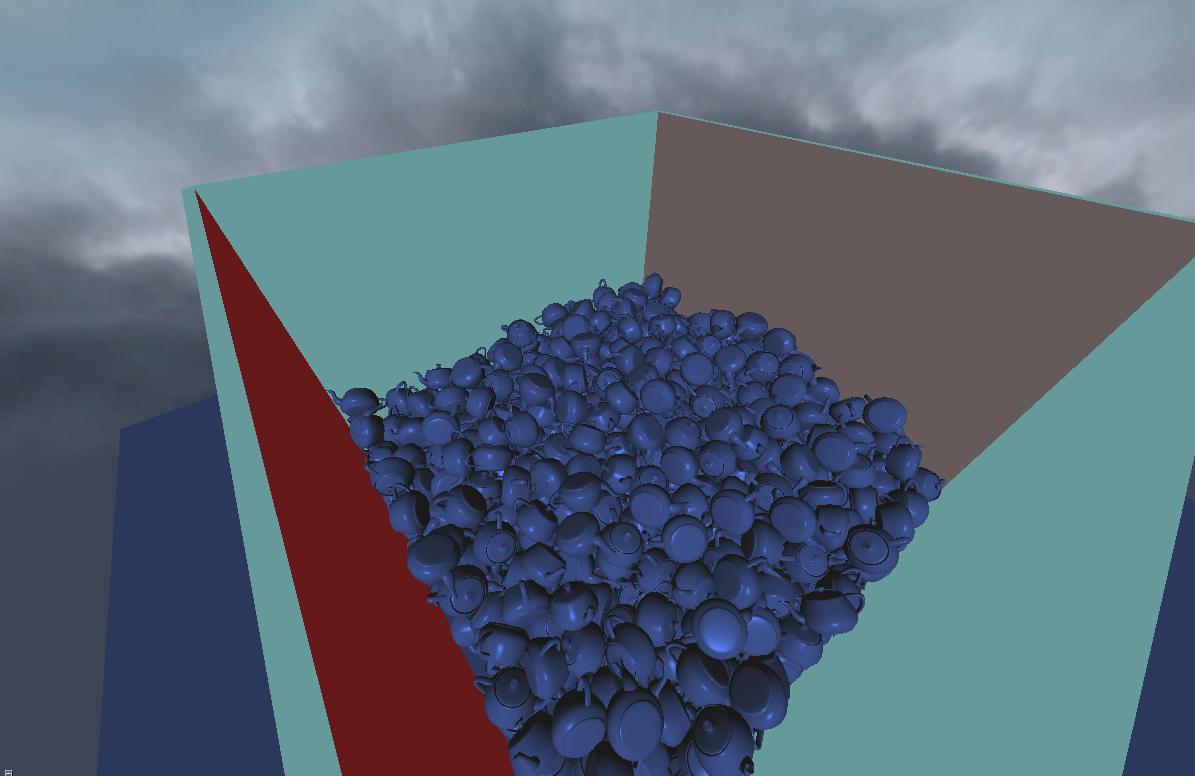
\includegraphics[width = 0.8\textwidth]{HACD512-05-11.png}
  \caption{The end result of the simulation}
  \label{fig:hacd0.0}
\end{figure}

\begin{figure}[H]
  \centering
  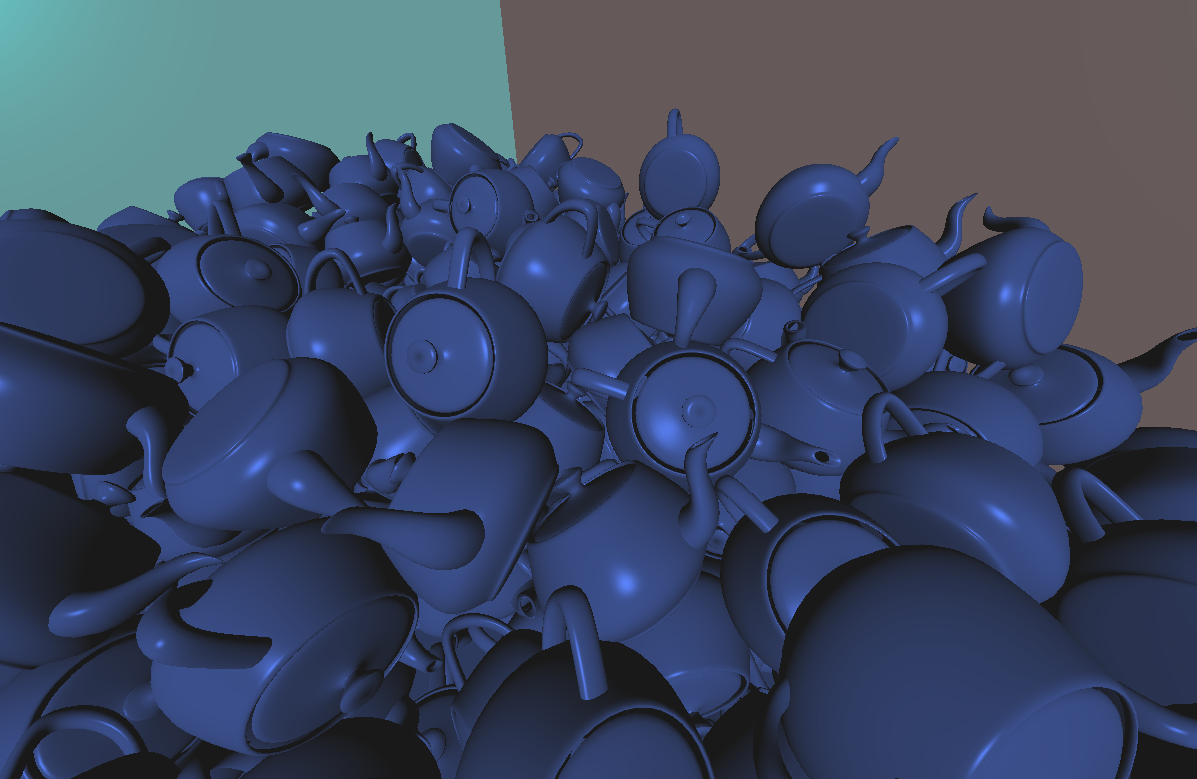
\includegraphics[width = 0.8\textwidth]{HACDtight.png}
  \caption{Close-up of finished result}
  \label{fig:tight}
\end{figure}

\section{Remarks}
While the time necessary for the decomposition renders it implausible for online uses
it is still an excellent tool for a preprocessing step, or a design step.
The models could be
decomposed at the start and copies of the same shape could be used, i.e. no additional
HACD's are performed. For this thesis the result were also saved to an Wavefront Object (.obj) file so simple and quick
 loading of the decomposed models could be used while testing.

The performance of the whole system simulation, while not phenomenal, is fast enough
for the generation of synthetic data, assuming that suitable simulation parameters
are selected.

The method does handle concave results through the approximate decomposition.

In terms of correctness the approximate decomposition, while good, does not reproduce the objects
perfectly.

%A concave collision result is portrayed in figure~\ref{fig:concaveHACD}.

\section{Limitations}
The limitations of this method are mainly concerning the performance. The fact
that the parameters of the HACD might affect the decomposition makes the system
as a whole less robust.
